

In the video lecture, we have seen a connection between functions $f: V \rightarrow V$
and trees on $V$. We used this to learn something about the number of such trees.
Here, we will go in the reverse direction: the connection will actually teach us a bit
about the number of functions with a special structure.\\

Let $V$ be a set of size $n$. We have learned that there are $n^n$ functions $f: V \rightarrow V$.
For such a function we can draw an ``arrow diagram" by simply drawing an arrow from
$x$ to $f(x)$ for every $V$. For example, let $V = \{0,\dots,7\}$ and $f(x) := x^2 \mod 8$.
The arrow diagram of $f$ looks as follows:
\begin{center}
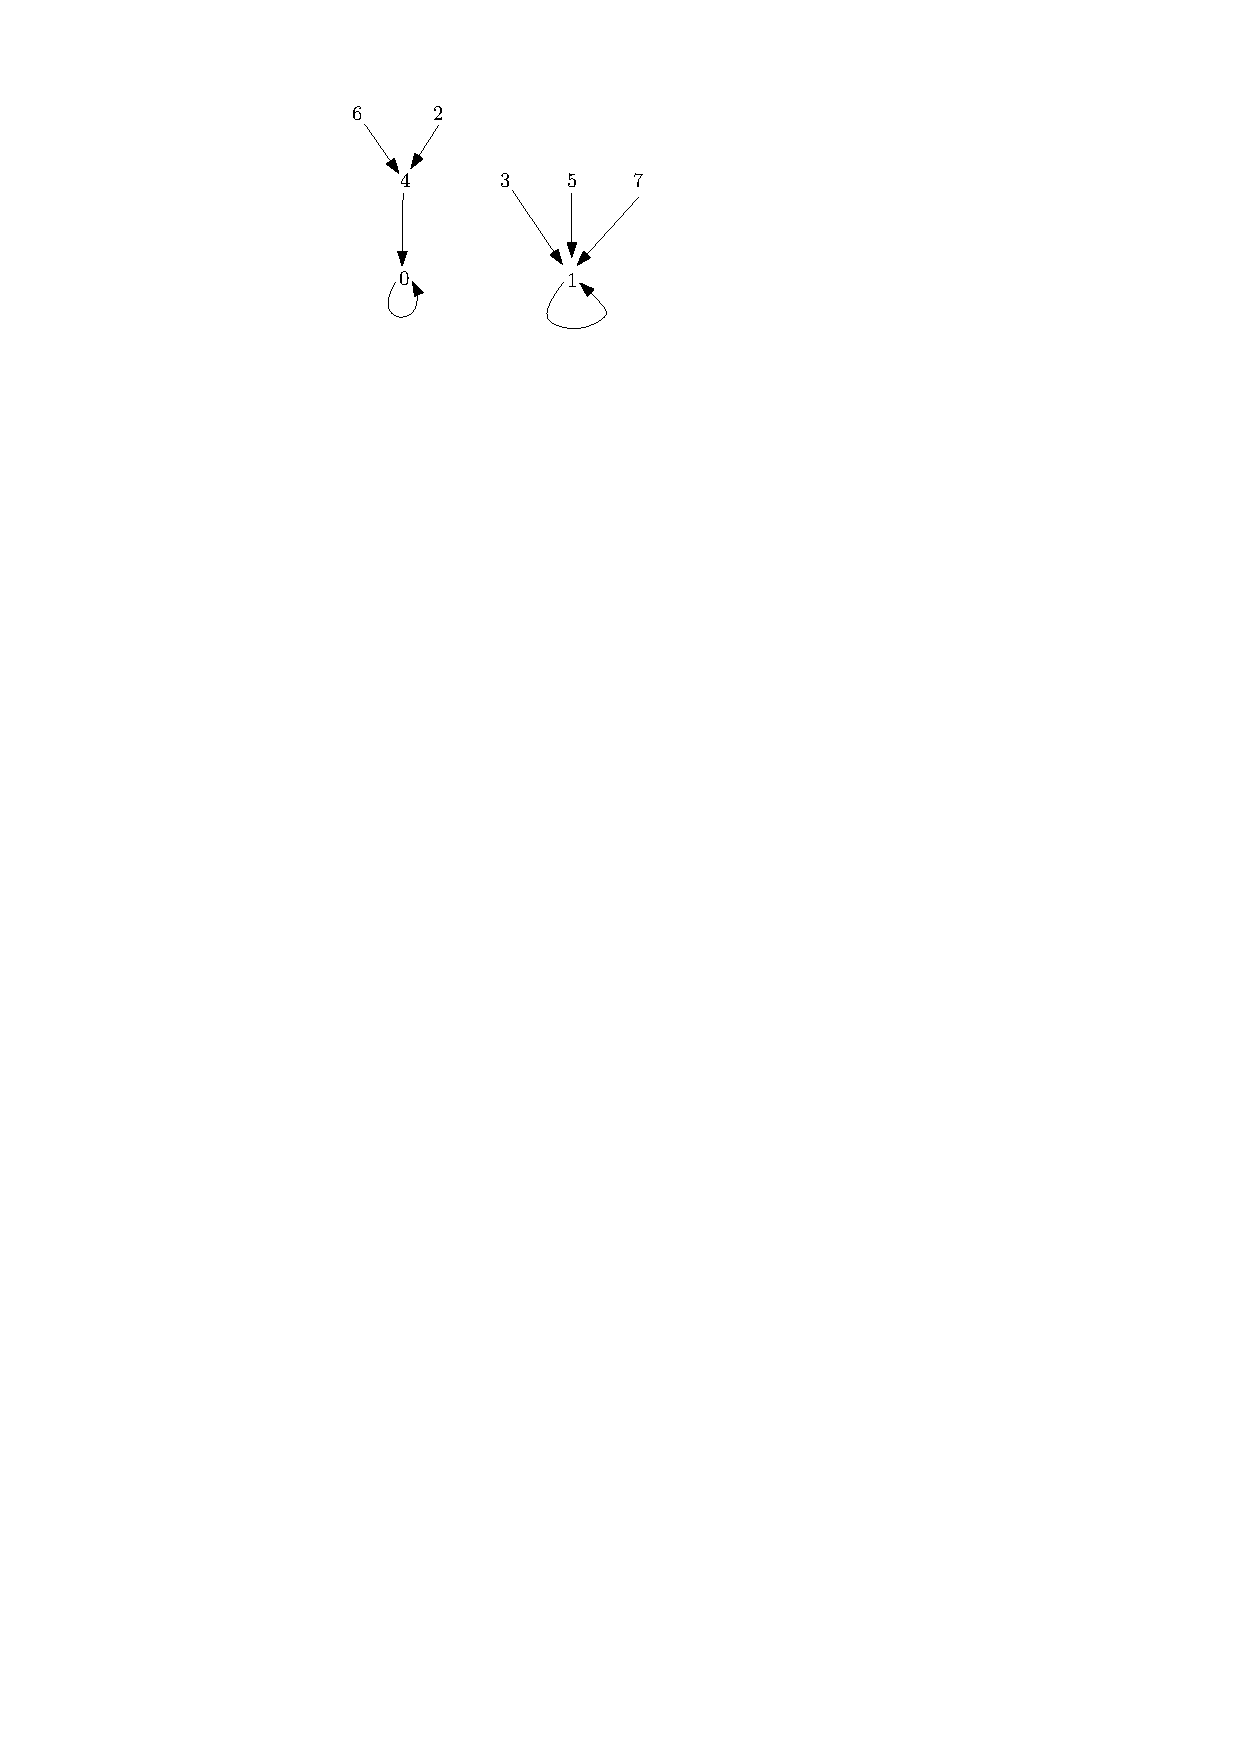
\includegraphics[width=0.3\textwidth]{figures/arrow-diagram.pdf}
\end{center}
The {\em core} of a function is the set of elements lying on cycles in such a diagram.
For example, the core of the above function is $\{0,1\}$. Formally, the core of $f$ is the
set
\begin{align*}
%\core(f) =
\{x \in V \ | \ \exists k \geq 1 f^{(k)}(x) = x \}
\end{align*}
where $f^{(k)}(x) = f( f( \dots f(x) \dots ))$, i.e., the function $f$ applied $k$ times
iteratively to $x$.

\begin{exercise}
Of the $n^n$ functions from $V$ to $V$, how many have a core of size $1$?
Give an explicit formula in terms of $n$.
\end{exercise}
\textbf{Solution.}
\par It is obvious that there are $n^{n-2}$ trees on $n$ vertices, with $n-1$ many edges. Because there is a function from $V$ to $V$, so there must be n edges in the graph. The one left forms a cycle and there are $n$ ways to choose the cycle because there are $n$ vertices. In total ,there are $n\times n^{n-2}= n^{n-1}$ functions.

\begin{exercise}
How many have a core of size $2$ that consists of two $1$-cycles? By this we mean
that $\core(f) = \{x,y\}$ with $f(x) = x$ and $f(y) = y$.
\end{exercise}
\textbf{Solution.}
\par This question is a little difficult because there is $n-2$ edges left regardless of the cycle. So let's divide the n vertices into $2$ parts(at least one vertex in a part) so there are $2^{n-1}-1$ ways to divide (because there is a symmetry). For each division, there are
\begin{equation*}
\tbinom{n}{2}
\end{equation*}
ways to choose the 2 left cycles. So the total number of functions is
\begin{equation*}
\tbinom{n}{2}\times (2^{n-1}-1)
\end{equation*}


\textbf{Hint.} For the previous two exercises, you need to use the link between functions
 $f: [n]\rightarrow [n]$ and
vertebrates $(T,h,b)$ from the video lecture.





\subsection{Counting Trees with Pr\"ufer Codes}

In the video lecture, we have seen Cayley's formula, stating that there are exactly
$n^{n-2}$ trees on the vertex set $[n]$. We showed a proof using
{\em vertebrates}. For this homework, read Section 7.4 of the textbook, titled
``A proof using the Pr\"ufer code''.


\begin{exercise}
  Let $V = \{1,\dots,9\}$ and consider the code $(1,3,3,2,6,6,1)$. Reconstruct a tree
  from this code. That is, find a tree on $V$ whose Pr\"ufer code is $(1,3,3,2,6,6,1)$.
\end{exercise}
\begin{center}
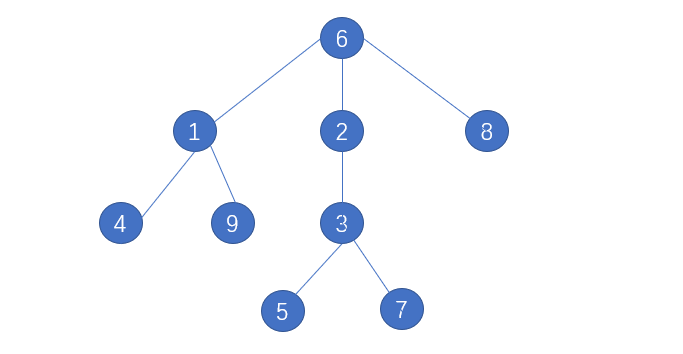
\includegraphics[width=0.3\textwidth]{./figures/prufer1.jpeg}
\end{center}
\begin{exercise}
  Let $\mathbf{p} = (p_1,p_2,\dots,p_{n-2})$ be the Pr\"ufer  code of some tree $T$ on $[n]$.
  Find a way to quickly determine the degree of vertex $i$ only by looking
  at $\mathbf{p}$ and not actually constructing the tree $T$.
  In particular, by looking at $\mathbf{p}$, what are the leaves of $T$?
\end{exercise}
\textbf{Solution.}
\par We assume the times vertex $i$ appear in the Pr\"ufer code is $i_t$, and it is obvious the degree of vertex is $i_t+1$ , and the the leaves of $T$ are the vertices which don't appear in the Pr\"ufer code.


